%==============================================================================
%  Measuring Muscle, Automatically
%  CSE 754 Computer Vision -- Course Project Report
%
%  Compile:  pdflatex main -> bibtex main -> pdflatex main -> pdflatex main
%  (or just press Recompile on Overleaf)
%
%  All figures live in ../figures/ and are produced by
%    scripts/make_figures.py  and  scripts/make_result_figures.py
%==============================================================================

\documentclass[11pt,a4paper]{article}

\usepackage[utf8]{inputenc}
\usepackage[T1]{fontenc}
\usepackage[margin=2.4cm]{geometry}
\usepackage{graphicx}
\usepackage{booktabs}
\usepackage{amsmath}
\usepackage{amssymb}
\usepackage{siunitx}
\usepackage{caption}
\usepackage{subcaption}
\usepackage{xcolor}
\usepackage{microtype}
\usepackage[numbers,sort&compress]{natbib}

\definecolor{NavyBlue}{HTML}{1D3557}
\definecolor{Accent}{HTML}{E07A1F}

\usepackage[colorlinks=true,linkcolor=NavyBlue,citecolor=NavyBlue,urlcolor=NavyBlue]{hyperref}
\usepackage{url}

\graphicspath{{../figures/}}

% Float placement: these figures are wide, and LaTeX's defaults strand them on
% half-empty pages. Loosen the fractions rather than forcing [H] everywhere.
\renewcommand{\topfraction}{0.92}
\renewcommand{\bottomfraction}{0.75}
\renewcommand{\textfraction}{0.08}
\renewcommand{\floatpagefraction}{0.75}
\setcounter{topnumber}{3}
\setcounter{totalnumber}{4}

\captionsetup{font=small,labelfont=bf}
\setlength{\parskip}{0.35em}

% Convenience macros -- edit these once and they update everywhere.
\newcommand{\MT}{\ensuremath{\mathrm{MT}}}
\newcommand{\PA}{\ensuremath{\mathrm{PA}}}
\newcommand{\FL}{\ensuremath{\mathrm{FL}}}
\newcommand{\degs}{\si{\degree}}

%==============================================================================
\begin{document}
%==============================================================================

%------------------------------------------------------------------ TITLE ----
\begin{titlepage}
\centering
\vspace*{2.5cm}

{\Huge\bfseries Measuring Muscle, Automatically\par}
\vspace{0.8em}
{\Large Geometry-aware deep learning for muscle architecture\\estimation in B-mode ultrasound\par}

\vspace{1.2cm}
{\color{Accent}\rule{0.55\textwidth}{1.2pt}}
\vspace{1.2cm}

{\large\bfseries CSE 754 --- Computer Vision\par}
{\large Course Project Report\par}

\vspace{2cm}

%--------------------------------------------------------------- GROUP INFO --
{\large\bfseries Group Information\par}
\vspace{0.6em}
\begin{tabular}{ll}
\toprule
\textbf{Name} & Shamima Hossain \\
\textbf{Student ID} & 21141119 \\
\textbf{Course} & CSE 754 --- Computer Vision \\
\textbf{Submission} & Final Project Report \\
\bottomrule
\end{tabular}

\vspace{1.4cm}

{\small
\begin{tabular}{r@{\hspace{1.2em}}l}
\textbf{Competition} & UMUD Challenge: Muscle Architecture in Ultrasound Data \\
\textbf{Public leaderboard} & \textbf{0.75306} (\texttt{UMUD\_score}, lower is better) \\
\textbf{Code} & \url{https://github.com/silvererudite/umud-muscle-architecture} \\
\end{tabular}}

\vfill
{\large \today\par}
\end{titlepage}

%--------------------------------------------------------------- ABSTRACT ----
\begin{abstract}
\noindent
Three parameters describe skeletal-muscle architecture --- muscle thickness,
pennation angle and fascicle length --- and all three are still measured by hand
from B-mode ultrasound, slowly and with substantial operator dependence. We
build a fully automatic pipeline for the UMUD challenge, which asks for these
three measurements on 309 held-out ultrasound frames.

The task turns out not to be the supervised regression problem it first appears
to be. The training data contains segmentation masks but \emph{no measurement
labels at all}, and no pixel-to-millimetre metadata, while two of the three
targets are physical lengths. The measurements must therefore be
\emph{reconstructed} geometrically, and the scale must be recovered by reading
the depth ruler that each scanner burns into its own images. We recognise six
scanner families and recover the scale on \textbf{100\,\%} of test frames, with
implied fields of view (\SIrange{2.97}{6.95}{\centi\metre} deep) matching the
manufacturers' documented presets.

Two U-Nets segment the aponeuroses and the fascicles, the latter carrying an
additional head that predicts a dense fascicle-orientation field as a
doubled-angle unit vector. A geometric module converts masks to measurements in
millimetre space. Because no frame carries an expert measurement, we introduce a
\emph{pseudo-ground-truth} protocol: the same geometry module is run on the
annotator's masks and on the network's, and the two are compared.

Held-out, the pipeline recovers muscle thickness to \textbf{0.3\,\%} and
pennation angle to \textbf{\ang{1.16}}; aponeurosis segmentation reaches a Dice
of \textbf{0.839}. On the competition leaderboard it scores \textbf{0.75306},
placing it just ahead of DL\_Track\_US, the tool currently used in this field.

We regard the negative results as the more valuable contribution. Of four
mechanisms proposed at the outset, the orientation head does not beat the
post-processing it was designed to replace, sequence smoothing is nearly inert,
and the per-frame confidence does not predict error. The fourth ---
reconstructing fascicle length by intersecting the fascicle with the fitted
aponeuroses --- does help, but \emph{not for the reason proposed}: on a
controlled comparison it loses to the textbook $\MT/\sin(\PA)$
($p=0.0003$), and it earns its place instead through boundedness against
$1/\sin$ ill-conditioning at shallow pennation angles. A rule that uses each
construction only where it is well conditioned improves the leaderboard score by
5\,\% relative over either alone.
\end{abstract}

\tableofcontents
\newpage

%----------------------------------------------------------- INTRODUCTION ----
\section{Introduction}

\subsection{Motivation}

B-mode ultrasound is cheap, portable and non-ionising, which makes it the
standard tool for imaging skeletal muscle in sports science, rehabilitation and
neuromuscular medicine. Three quantities summarise the internal architecture of
a pennate muscle (Figure~\ref{fig:geometry}):

\begin{itemize}
  \item \textbf{muscle thickness} (\MT, \si{\milli\metre}) --- the separation of
        the superficial and deep aponeuroses;
  \item \textbf{pennation angle} (\PA, \degs) --- the angle between a muscle
        fascicle and the deep aponeurosis;
  \item \textbf{fascicle length} (\FL, \si{\milli\metre}) --- the length of a
        fascicle between the two aponeuroses.
\end{itemize}

These are still obtained by an operator drawing lines on a screen. The procedure
is slow, subjective, and dependent on experience. Automated tools exist ---
DL\_Track\_US~\citep{ritsche2024dltrack} is the most widely used --- but their
own authors report that accuracy is not yet sufficient for out-of-the-box
use~\citep{ritsche2026umud}.

\subsection{Task}

The UMUD challenge~\citep{umudchallenge2026} provides 309 test frames and asks
for all three parameters per frame. Submissions are scored by a custom
\texttt{UMUD\_score} (lower is better), with 33\,\% of rows on the public
leaderboard and 67\,\% held back.

\subsection{What makes this hard}

Five properties of the data, none of them visible from the task description,
dominate the engineering. They are established empirically in
Section~\ref{sec:data}.

\begin{enumerate}
  \item \textbf{There are no measurement labels.} The training data provides
        masks --- aponeurosis bands and fascicle segments --- and never a
        thickness or an angle. The targets must be derived geometrically, and so
        must any offline validation signal.
  \item \textbf{There is no scale metadata.} Two targets are in millimetres; the
        network sees pixels. The conversion must be read off the scanner's
        burnt-in depth ruler, and every scanner family draws it differently.
  \item \textbf{The fascicle annotations are segments, not fascicles.}
        Annotators traced the locally visible portion of a representative sample
        of fascicles. They are a poor length target and an excellent
        \emph{orientation} target.
  \item \textbf{70\,\% of training frames disagree in size with their own mask.}
  \item \textbf{26\,\% of the fascicle training images are duplicates} of another
        image in the same set.
\end{enumerate}

Points 4 and 5 are silent failure modes: neither raises an error, and both
corrupt results in ways that resemble success.

\subsection{Contributions}

\begin{enumerate}
  \item A complete, reproducible pipeline --- ruler calibration, segmentation,
        geometric reconstruction --- scoring \textbf{0.75306} on the public
        leaderboard, ahead of the field's reference tool.
  \item A \textbf{scale-recovery module} that reads the depth ruler of six
        scanner families and succeeds on 100\,\% of test frames, validated
        against documented hardware presets.
  \item A \textbf{pseudo-ground-truth evaluation protocol} that makes offline
        model selection possible in a task with no measurement labels and a
        five-submissions-per-day budget.
  \item A set of \textbf{negative and corrective results} (Section~\ref{sec:disc})
        obtained by measuring each proposed mechanism against the thing it was
        meant to replace --- including the finding that a more faithful geometric
        model can be a \emph{worse} estimator when it depends on noisier inputs.
\end{enumerate}

%------------------------------------------------------ LITERATURE REVIEW ----
\section{Literature Review and Background}

\subsection{Automated muscle-architecture analysis}

\textbf{DL\_Track\_US}~\citep{ritsche2024dltrack} is the reference baseline and
the direct ancestor of this work: two U-Nets segment aponeuroses and fascicles,
and the architecture parameters are computed from the resulting masks by
post-processing. The training sets released with it are exactly the sets used in
this challenge. Its authors report a residual accuracy gap, particularly on video
sequences. \textbf{Marzola et al.}~\citep{marzola2021segmentation} segment
transverse musculoskeletal ultrasound across 3\,917 images and three muscles,
providing the main published evidence on cross-muscle and cross-device
generalisation --- the question our Section~\ref{sec:generalisation} revisits.
\textbf{Leitner et al.}~\citep{leitner2022mtj} track the muscle--tendon junction
across devices and subjects, and motivated the temporal component of our original
proposal.

The \textbf{UMUD} index~\citep{ritsche2026umud} aggregates 14 musculoskeletal
ultrasonography datasets ($\sim$76\,000 images, $\sim$2\,700 videos,
$\sim$1\,900 participants) and is the source of this challenge. It also indexes
a multi-expert set (35 images analysed independently by six operators) that would
be needed to calibrate uncertainty against human disagreement; that set is
\emph{not} part of the competition data, which is why the corresponding component
of our proposal could not be attempted.

\subsection{Segmentation architectures}

\textbf{U-Net}~\citep{ronneberger2015unet} remains the encoder--decoder backbone
of essentially every published baseline in this field, and we adopt it
deliberately: the aim of this project is not a better segmenter but a better way
of converting a segmentation into a measurement. We pair it with a
\textbf{ResNet-34}~\citep{he2016resnet} encoder initialised on
\textbf{ImageNet}~\citep{deng2009imagenet}.
\textbf{Segment Anything}~\citep{kirillov2023sam} was considered as a promptable
foundation-model alternative; with 1\,048 and 2\,761 annotated frames available
and a two-day budget, fine-tuning a conventional U-Net was the better use of
compute, and SAM is left as future work.

\subsection{Orientation estimation}

Fascicle direction is classically recovered \emph{after} segmentation, by a Hough
transform or by the \textbf{structure tensor}~\citep{knutsson1989tensor}. Our
proposal argued that orientation should instead be a first-class network output.
Both routes are implemented here and compared directly in
Section~\ref{sec:abl-orientation}.

An important technical point recurs throughout: orientation is a \emph{director},
not a vector. An angle $\theta$ and $\theta+\ang{180}$ describe the same
fascicle. Regressing $\theta$ directly makes the target discontinuous wherever it
crosses $\pm\ang{90}$, and arithmetic means of angles are simply wrong. Working
in doubled-angle coordinates $(\cos 2\theta, \sin 2\theta)$ removes both
problems.

\subsection{Temporal modelling}

\textbf{RAFT}~\citep{teed2020raft} provides dense optical flow by iterative
refinement and was the intended basis for propagating fascicle geometry across
video frames. The competition ships still images rather than video, so this was
re-scoped --- see Section~\ref{sec:sequence}.

%-------------------------------------------------------------- DATA -----
\section{Data}
\label{sec:data}

\begin{table}[htbp]
\centering
\caption{Competition data. ``Distinct'' counts unique images after
content hashing.}
\label{tab:data}
\begin{tabular}{lrrl}
\toprule
\textbf{Set} & \textbf{Files} & \textbf{Distinct} & \textbf{Annotation} \\
\midrule
Aponeurosis & 1\,048 & 1\,028 & superficial + deep bands \\
Fascicle    & 2\,761 & 2\,046 & short fascicle segments \\
\textit{Both} & \textit{78} & \textit{78} & used as the end-to-end validation set \\
Test        & 309   & 309   & none \\
\bottomrule
\end{tabular}
\end{table}

\begin{figure}[htbp]
\centering
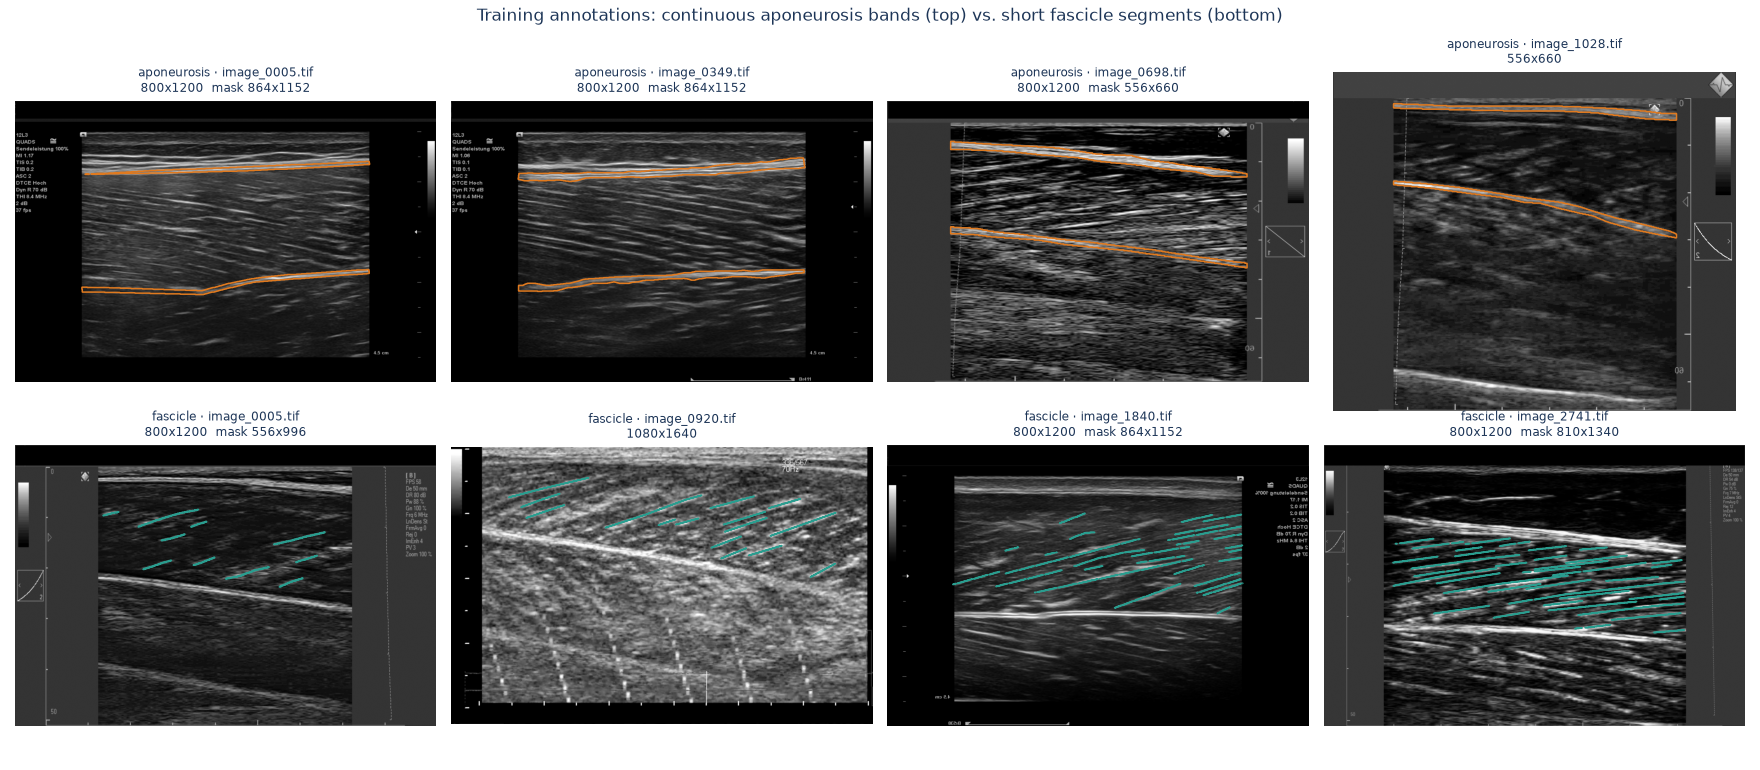
\includegraphics[width=\textwidth]{data_overview.png}
\caption{Training annotations. Top: continuous aponeurosis bands. Bottom: short
fascicle \emph{segments} --- annotators traced a representative sample, not every
fascicle, which is why Dice is a partly inappropriate metric for this task
(Section~\ref{sec:res-seg}).}
\label{fig:data}
\end{figure}

\subsection{Resolving the image/mask size mismatch}

Whenever image and mask disagree in size, the image is $800\times1200$ and the
mask is something else. Two readings are possible --- the mask is a \emph{crop}
of the image, or the image is a \emph{resize} of the mask's frame --- and they
imply opposite corrections. We tested it directly by resizing the mask onto the
image canvas and measuring mean image intensity beneath it. Aponeuroses are
bright, so a correctly aligned mask should sit on high intensity.

\begin{table}[htbp]
\centering
\caption{Mask--image alignment test, $n=300$ sampled pairs.}
\label{tab:alignment}
\begin{tabular}{lr}
\toprule
& \textbf{Mean intensity under mask $\div$ frame mean} \\
\midrule
Shape-matched pairs                        & 3.09 \\
Shape-mismatched pairs, after plain resize & \textbf{3.71} \\
Control (same mask rolled by a quarter frame) & 1.25 \\
\bottomrule
\end{tabular}
\end{table}

The mismatched pairs align at least as well as the matched ones after a plain
resize, and far better than the deliberately misaligned control. The image is a
resize of the mask's frame; resampling both onto a common canvas restores the
correspondence.

\subsection{Duplicate leakage}

Splitting the fascicle set at random places \textbf{179 content groups on both
sides} of the train/validation boundary: the model would be validated on frames
it had trained on. Our splitter assigns whole content groups, stratified by
acquisition shape, reducing the leak to zero (Table~\ref{tab:split}).

\begin{table}[htbp]
\centering
\caption{Content groups leaking across the train/validation split.}
\label{tab:split}
\begin{tabular}{lrr}
\toprule
\textbf{Task} & \textbf{Naive random split} & \textbf{Content-grouped split} \\
\midrule
Aponeurosis & 2   & \textbf{0} \\
Fascicle    & 179 & \textbf{0} \\
\bottomrule
\end{tabular}
\end{table}

\begin{figure}[htbp]
\centering
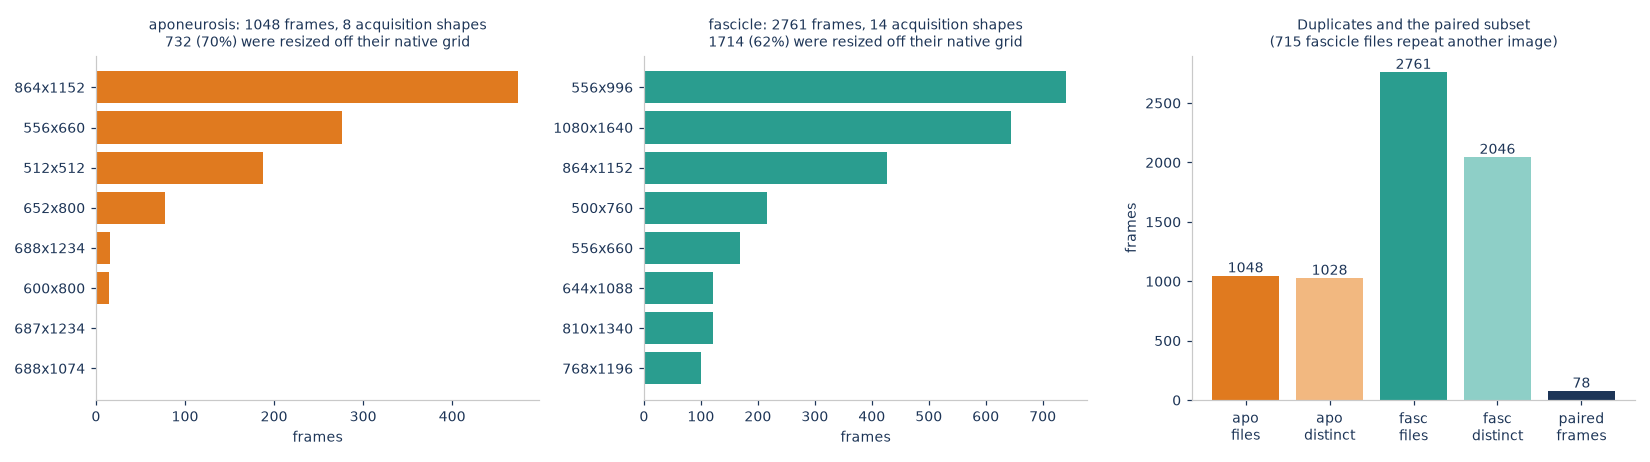
\includegraphics[width=\textwidth]{dataset_stats.png}
\caption{Acquisition shapes, resizing, duplicates and the paired subset.}
\label{fig:stats}
\end{figure}

%------------------------------------------------------------ METHODOLOGY ----
\section{Methodology}
\label{sec:method}

The pipeline is:
\begin{center}
frame $\rightarrow$ ruler calibration $\rightarrow$ two U-Nets $\rightarrow$
geometric reconstruction $\rightarrow$ sequence consensus $\rightarrow$
$(\PA,\FL,\MT)$
\end{center}

\subsection{Scale calibration}
\label{sec:calibration}

Every target is physical but the network sees pixels, and the competition
supplies no scale. The conversion is recovered from the depth ruler each scanner
draws into its own image. Our module dispatches on frame shape plus a signature
pixel to identify one of six scanner families, reads the tick pitch from the
appropriate margin, and falls back to a generic autocorrelation ruler detector
otherwise. The per-family tick geometry follows the public analysis of
AmbrosM~\citep{ambrosm2026quickdirty}; which pixel column a given scanner uses is
an empirical fact about the data rather than something derivable, and we cite it
rather than re-derive it.

\paragraph{Result.} \textbf{100\,\% of the 309 test frames calibrate.} The
recovered scales pass an independent plausibility check: implied fields of view
span \SIrange{2.97}{6.95}{\centi\metre} in depth and
\SIrange{2.84}{6.41}{\centi\metre} laterally, matching the documented
\SIrange{3}{7}{\centi\metre} depth presets and the \SI{2.85}{\centi\metre} /
\SI{5.75}{\centi\metre} sector widths of the two dominant probes. Nothing in the
procedure was fitted to those numbers, so the agreement is evidence rather than
circularity.

\paragraph{A guard worth recording.} An early version of the generic fallback
invented a scale for images that have \emph{no} ruler --- the $512\times512$
training crops --- by locking onto border speckle, returning
49\,px/cm where the device table gives 77.8. That
$1.6\times$ error inflated every millimetre downstream. The detector now requires
the strip to look like scanner chrome (dark background, short bright runs) and
the tick gaps to be regular to within 12\,\%; \emph{a wrong scale is worse than
no scale}, so it now reports failure instead. Honest coverage on training data is
60\,\% (aponeurosis) and 12\,\% (fascicle), which is precisely why the offline
evaluation of Section~\ref{sec:protocol} is scale-free.

\begin{figure}[htbp]
\centering
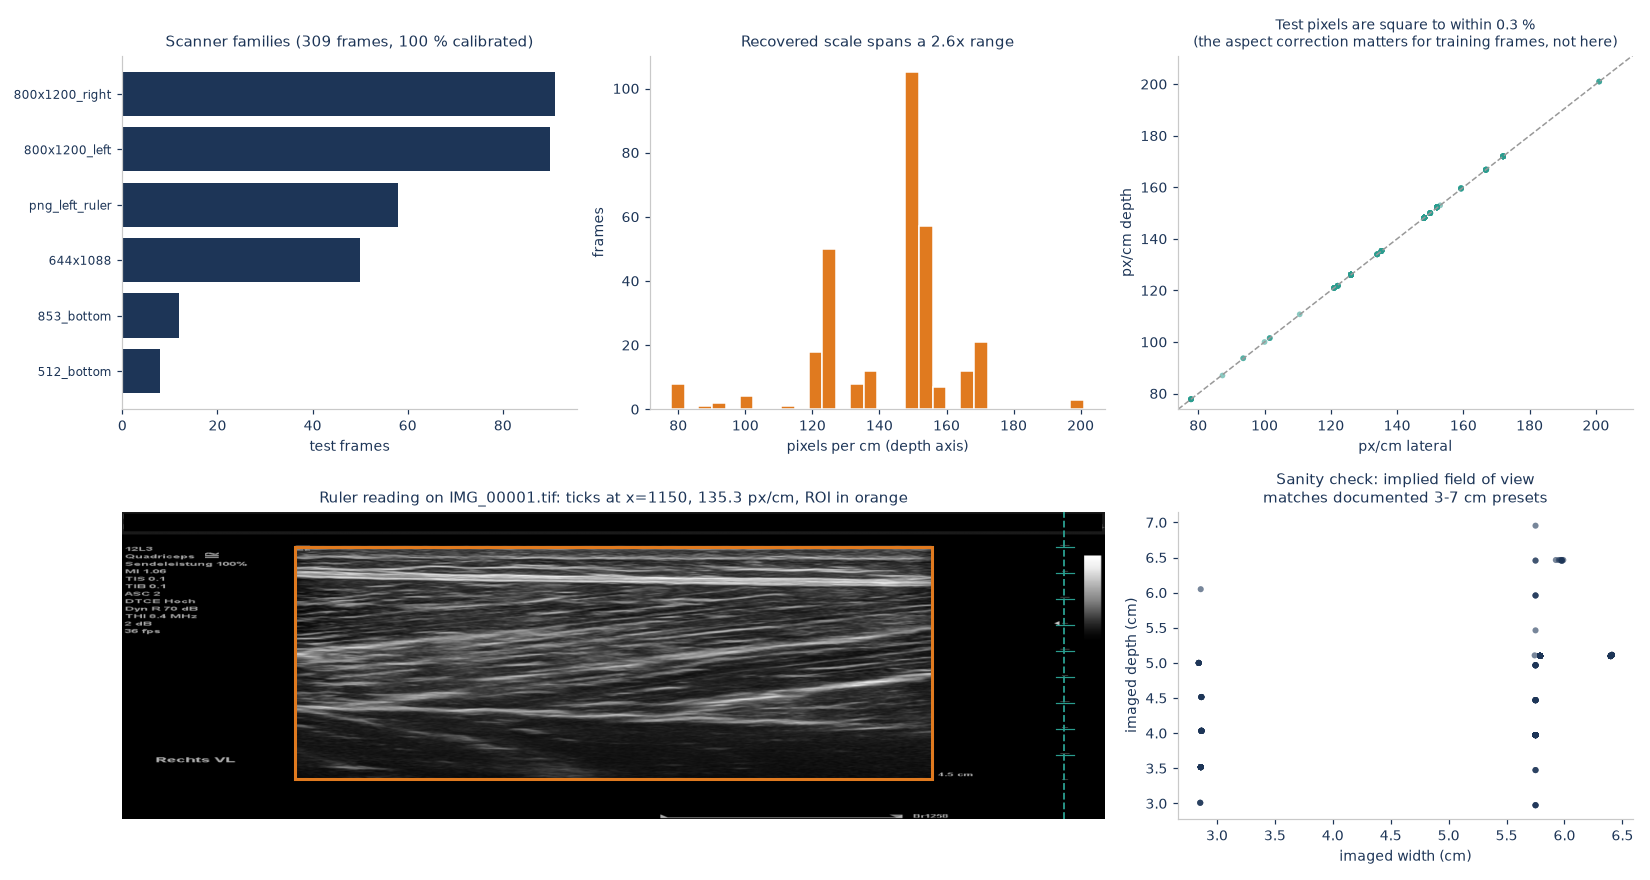
\includegraphics[width=\textwidth]{calibration.png}
\caption{Scanner families, recovered scales, and the ruler-reading procedure.
Bottom right: implied field of view, an independent check that was not fitted.}
\label{fig:calibration}
\end{figure}

\begin{figure}[htbp]
\centering
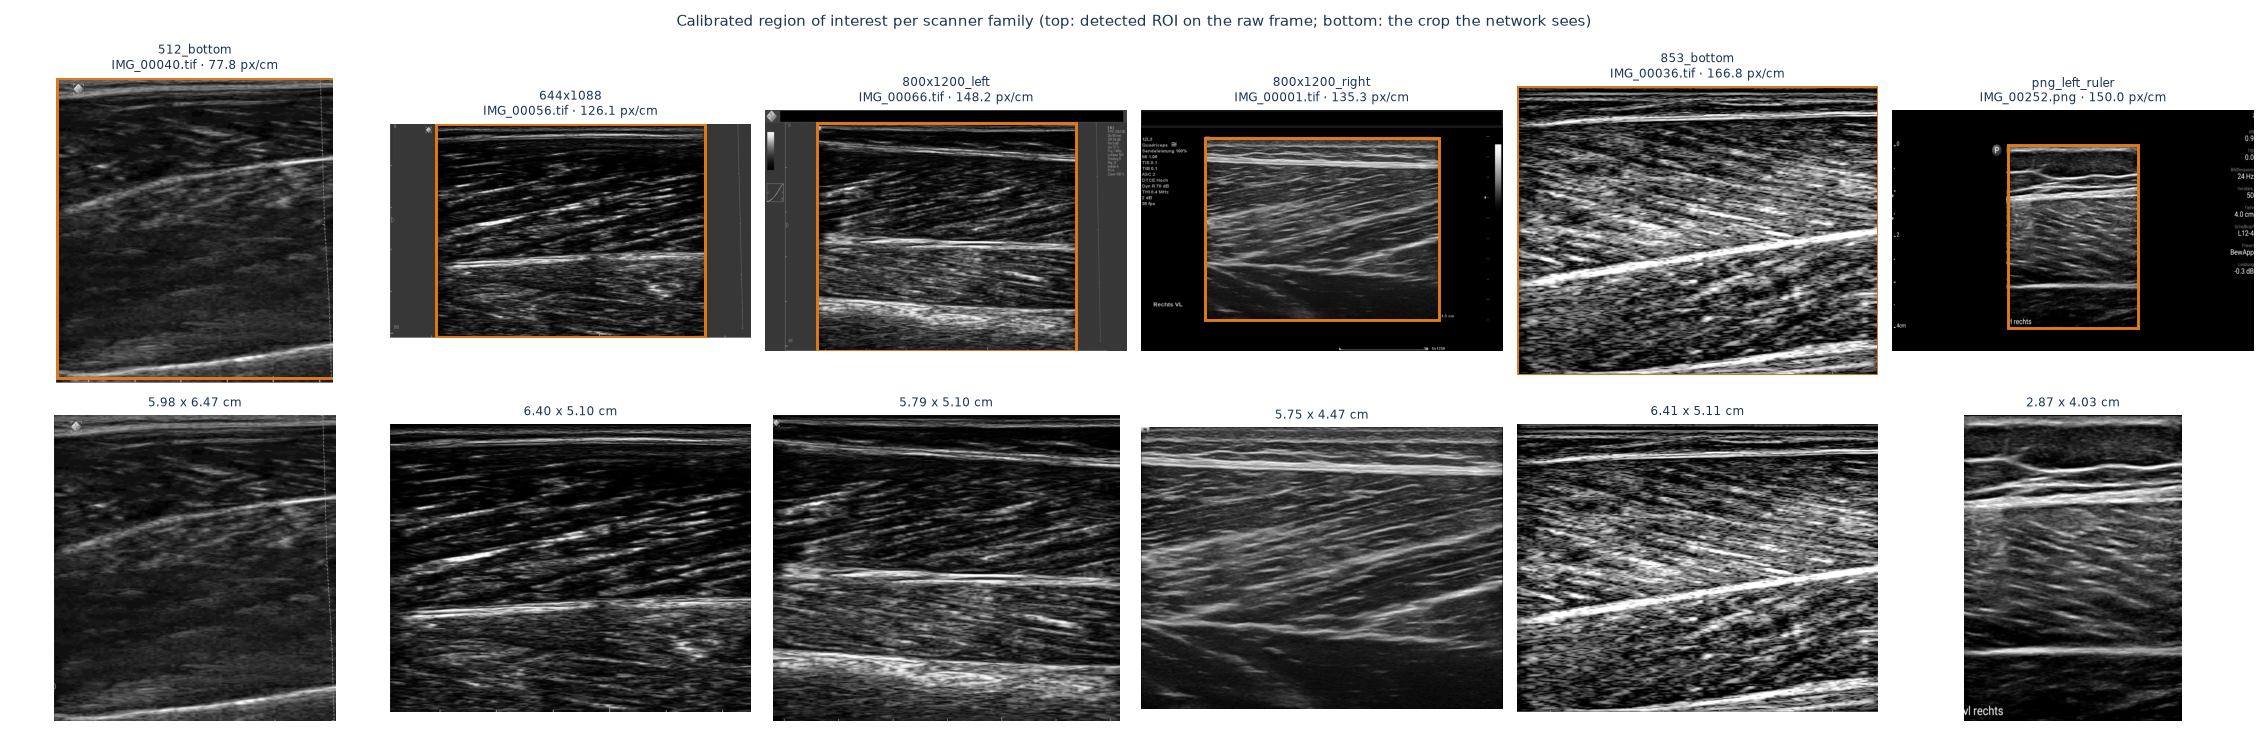
\includegraphics[width=\textwidth]{roi_by_family.png}
\caption{Calibrated region of interest for all six scanner families. Top: the
detected ROI on the raw frame. Bottom: the crop the network sees, with its
physical size. Everything downstream depends on this being correct.}
\label{fig:roi}
\end{figure}

\subsection{Segmentation networks}

Two U-Nets~\citep{ronneberger2015unet} over an ImageNet-initialised ResNet-34
encoder~\citep{he2016resnet}, one for aponeuroses and one for fascicles. B-mode
ultrasound is grayscale, so rather than tiling the channel we sum the pretrained
RGB stem weights, which preserves filter response exactly for a gray input.
Input $512\times512$, batch 8, AdamW with one-cycle scheduling, mixed precision,
and a loss of $\tfrac12\,\text{BCE} + \tfrac12\,\text{Dice}$. Dice matters here
because the positive class occupies 0.3--3\,\% of a frame, placing the pure-BCE
optimum uncomfortably close to predicting background everywhere.

\paragraph{Augmentation.} Deliberately minimal: horizontal flip --- a mirrored
scan is a scan of the other leg, and its effect on the orientation field is
exactly invertible --- plus gain and gamma jitter standing in for scanner preset
differences. \textbf{No vertical flip and no rotation}: a vertical flip would
place the deep aponeurosis above the superficial one, inverting the anatomy the
geometry module relies on, and pennation angle is defined relative to the probe
axis.

\subsection{The orientation head}
\label{sec:orientation}

The fascicle network carries a second output head predicting a dense orientation
field as a doubled-angle unit vector $(\cos 2\theta, \sin 2\theta)$ per pixel.
Aggregation over a frame uses circular statistics,
\begin{equation}
\bar\theta = \tfrac12 \operatorname{atan2}\!
  \left( \sum_i w_i \sin 2\theta_i,\; \sum_i w_i \cos 2\theta_i \right),
\label{eq:circmean}
\end{equation}
with $w_i$ the segmentation confidence. The resultant length
$R=\lVert \sum_i w_i (\cos 2\theta_i, \sin 2\theta_i) \rVert / \sum_i w_i$
comes free as a dispersion measure.

The loss is a masked cosine distance, $1-\langle \hat{\mathbf{u}},
\mathbf{u}\rangle$, which equals $1-\cos 2\Delta\theta$ and is therefore blind to
the physically meaningless $\ang{180}$ flip. It is evaluated \emph{only} where an
annotator drew a fascicle; orientation is undefined in the surrounding speckle,
and supervising it there teaches the head to regress background texture.

\paragraph{Validating a derived target.} The supervision is derived from the
masks by a structure tensor, not annotated, so it requires its own check. Against
an independent per-segment principal-axis estimator over 60 random frames, the
targets agree to a \textbf{median of \ang{1.10}, with 100\,\% of frames within
\ang{5}}.

\subsection{Geometric reconstruction}
\label{sec:geometry}

All geometry is solved in millimetre space, correcting for pixel aspect ratio
before any angle is measured. Aponeuroses are fitted as low-order polynomials
rather than straight lines, since a visible fraction of frames show curvature.
Thickness is the median perpendicular separation over the span where both curves
are defined. Pennation angle is referenced to the \emph{deep aponeurosis}, which
is what the clinical definition specifies, rather than to the image horizontal.

Fascicle length is computed two ways:
\begin{align}
\FL_{\text{textbook}} &= \frac{\MT}{\sin \PA}, \label{eq:textbook}\\[2pt]
\FL_{\text{intersection}} &= \lVert \mathbf{p}_{\text{deep}} -
  \mathbf{p}_{\text{sup}} \rVert, \label{eq:intersect}
\end{align}
where in \eqref{eq:intersect} the fascicle ray is launched from the deep
aponeurosis and intersected with the locally linearised superficial aponeurosis.
Equation~\eqref{eq:textbook} assumes the two aponeuroses are parallel; they are
not, diverging by \ang{1.72} at the median with 42\,\% of frames exceeding
\ang{2}. Our proposal argued that \eqref{eq:intersect} should therefore be
preferred. \textbf{Section~\ref{sec:abl-fl} shows that this does not follow},
and the shipped default is a rule that selects between them.

\begin{figure}[htbp]
\centering
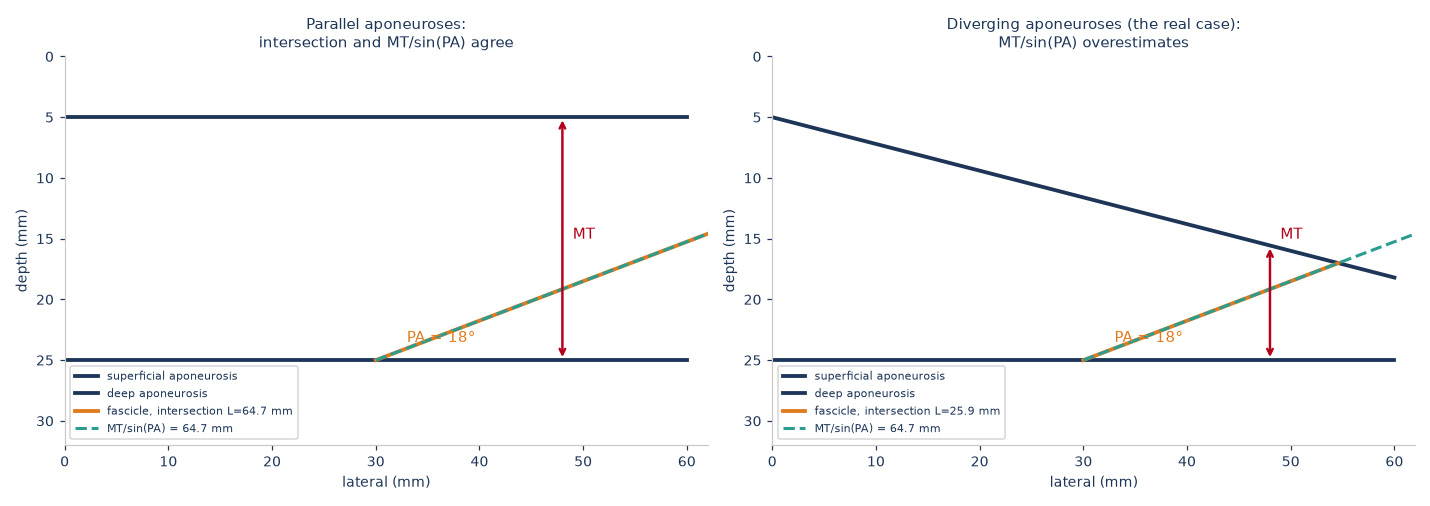
\includegraphics[width=\textwidth]{geometry_reconstruction.png}
\caption{The two fascicle-length constructions. Right panel drawn at the
\emph{measured} p90 aponeurosis divergence (\ang{3.1}), not an exaggeration:
the textbook ray overshoots the superficial aponeurosis by 17\,\%.}
\label{fig:geometry}
\end{figure}

\subsection{Sequence coherence}
\label{sec:sequence}

The proposal assumed video; the competition ships still frames. Rather than drop
the component, we recovered the latent structure: grouping by ROI-cropped
appearance, scanner family and depth setting reveals \textbf{27 runs of exactly
five consecutive frames} (135 frames) interleaved with 174 singletons. The
similarity distribution is sharply bimodal --- above 0.99 within runs, below 0.65
everywhere else --- so the grouping threshold sits in an empty gap and is not a
tuned parameter. Within a run, each parameter is replaced by a
confidence-weighted \emph{median}, robust to a single collapsed segmentation.

\begin{figure}[htbp]
\centering
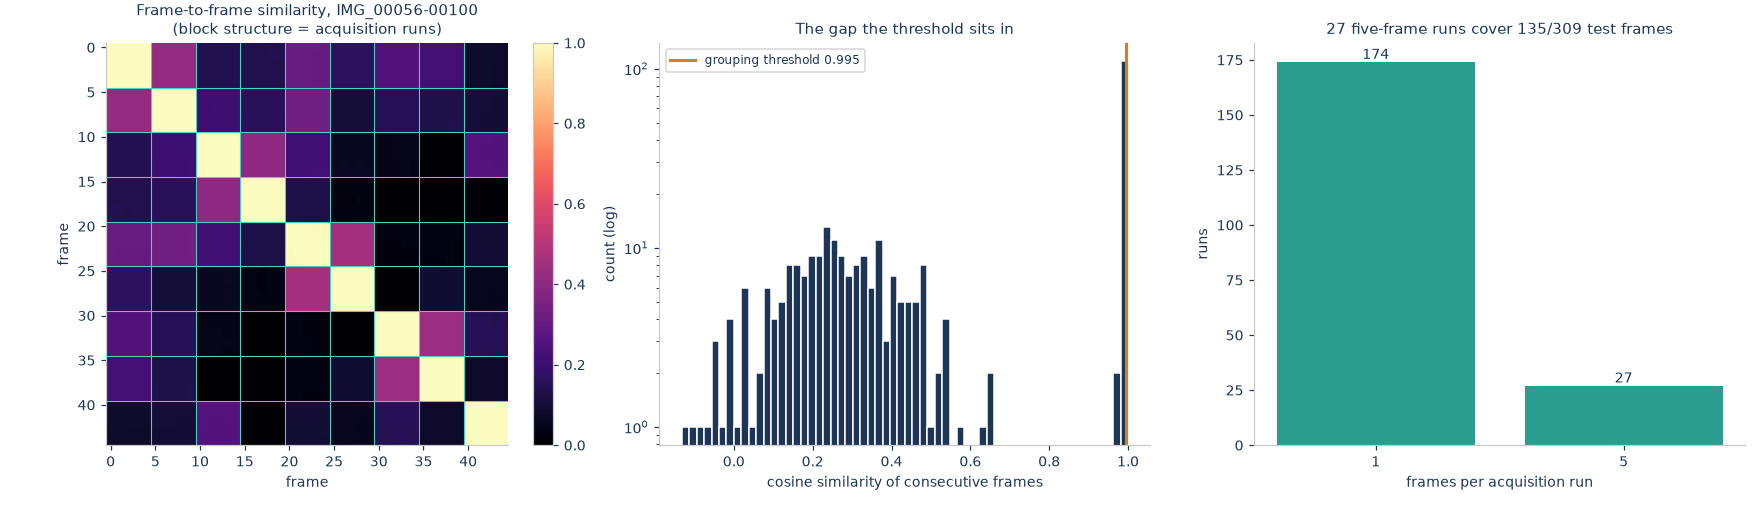
\includegraphics[width=\textwidth]{sequence_structure.png}
\caption{Recovering acquisition runs. Left: block structure in the
frame-similarity matrix. Middle: the empty gap the threshold sits in. Right: 27
five-frame runs cover 135 of 309 test frames.}
\label{fig:sequence}
\end{figure}

\subsection{Evaluation protocol}
\label{sec:protocol}

With no measurement labels and five submissions per day, design choices cannot be
made on the leaderboard. We therefore use a \textbf{pseudo-ground-truth}
protocol: run the \emph{same} geometric reconstruction twice, once on the
annotator's masks and once on the network's, and compare.

This measures the error the segmentation contributes, with the geometry module
held fixed. It does \emph{not} measure the error of the geometry module against a
human measurement --- that would require the expert-annotated UMUD subsets, which
are outside this competition's data. \textbf{This report therefore makes no claim
of agreement with expert measurement.}

Metrics are reported scale-free (lengths as a fraction of frame height, angles in
degrees on the frame's own grid), because the ruler survives the competition's
resizing on some training families and not others, and mixing calibration error
into a number meant to isolate segmentation would contaminate it.

\paragraph{An external check.} Pennation angle is scale-invariant, so running the
reconstruction on annotator masks yields a number comparable with the outside
world without trusting our calibration at all: it lands at a
\textbf{median of \ang{17.0}}, against a published range of \ang{10}--\ang{25}
for vastus lateralis and \ang{16.4} for an independent public leaderboard entry
built by a completely different pipeline~\citep{dread2026vera}. Two independent
routes agreeing to \ang{0.6} is the strongest available evidence that the
reconstruction is not systematically wrong.

%--------------------------------------------------- RESULTS AND DISCUSSION --
\section{Results and Discussion}
\label{sec:results}

\subsection{Segmentation}
\label{sec:res-seg}

Both models trained on a Kaggle T4 GPU, 93.6 minutes for the pair.

\begin{table}[htbp]
\centering
\caption{Segmentation performance on the content-grouped held-out split.}
\label{tab:seg}
\begin{tabular}{lrr}
\toprule
& \textbf{Aponeurosis} & \textbf{Fascicle} \\
\midrule
Training frames        & 893   & 2\,344 \\
Held-out frames        & 155   & 417 \\
Best epoch / total     & 29/45 & 16/35 \\
\textbf{Validation Dice} & \textbf{0.839} & \textbf{0.274} \\
Validation IoU         & 0.731 & 0.161 \\
Orientation-field error & ---   & \textbf{\ang{2.74}} \\
\bottomrule
\end{tabular}
\end{table}

\paragraph{Reading the fascicle Dice correctly.} A Dice of 0.27 is low, and the
metric is partly inappropriate rather than the model being poor. Annotators
traced a \emph{representative sample} of fascicles --- roughly a dozen short
segments in a field containing hundreds. A model that segments a different but
equally valid set is penalised by Dice while being exactly right for the purpose
the masks serve. The metric that reflects that purpose is the orientation error,
which reaches \ang{2.74}. The aponeurosis task carries no such ambiguity ---
there are exactly two bands and the annotator traced both --- and there Dice
reaches 0.839.

The fascicle model overfits after epoch 16 (Figure~\ref{fig:curves}): training
loss continues to fall while validation loss turns upward. Checkpointing on
validation Dice rather than on the final epoch is what keeps this out of the
submission.

\begin{figure}[htbp]
\centering
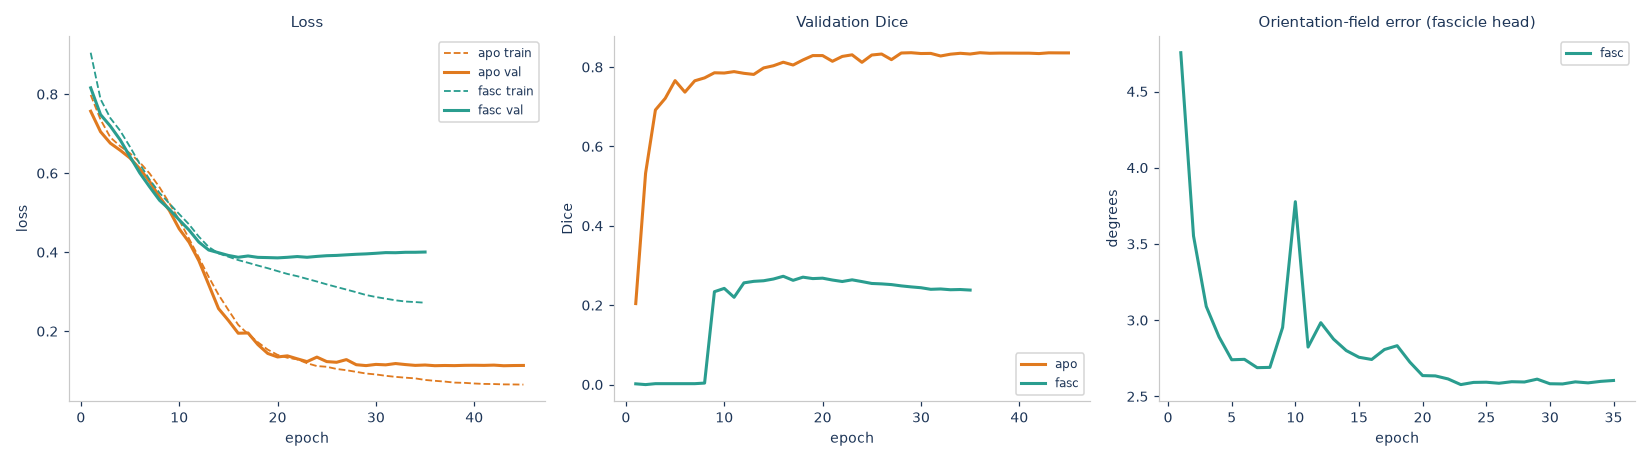
\includegraphics[width=\textwidth]{training_curves.png}
\caption{Training curves. The fascicle model overfits after epoch 16; the
orientation-field error plateaus near \ang{2.6}.}
\label{fig:curves}
\end{figure}

\subsection{Geometry (pseudo-ground-truth)}

\begin{table}[htbp]
\centering
\caption{End-to-end geometry error on the 78 frames carrying both annotations,
predicted masks versus annotator masks through the same geometry module.}
\label{tab:geom}
\begin{tabular}{lrrr}
\toprule
\textbf{Parameter} & \textbf{Median} & \textbf{Mean} & \textbf{p90} \\
\midrule
Muscle thickness (relative) & \textbf{0.003} & 0.059 & 0.059 \\
Pennation angle             & \textbf{\ang{1.16}} & \ang{1.66} & \ang{3.30} \\
Fascicle length (relative)  & \textbf{0.060} & 0.128 & 0.260 \\
\bottomrule
\end{tabular}
\end{table}

Thickness is the standout: the geometry recovers it from \emph{predicted} masks
to within 0.3\,\% of what it recovers from the annotator's own masks. That single
fact drives the most important design decision in the project
(Section~\ref{sec:abl-fl}). Aponeurosis divergence --- the quantity the
intersection construction rests on --- is also recovered well: \ang{1.68}
predicted against \ang{1.72}, median error \ang{0.15}.

\paragraph{Caveat.} All 78 paired frames are $512\times512$ crops from a
\emph{single} scanner family. They are the only frames carrying both
annotations, so this is the only end-to-end evidence available, but it says
nothing about how the two models behave together on the other five families ---
a limitation that Section~\ref{sec:abl-fl} shows to be consequential.

\begin{figure}[htbp]
\centering
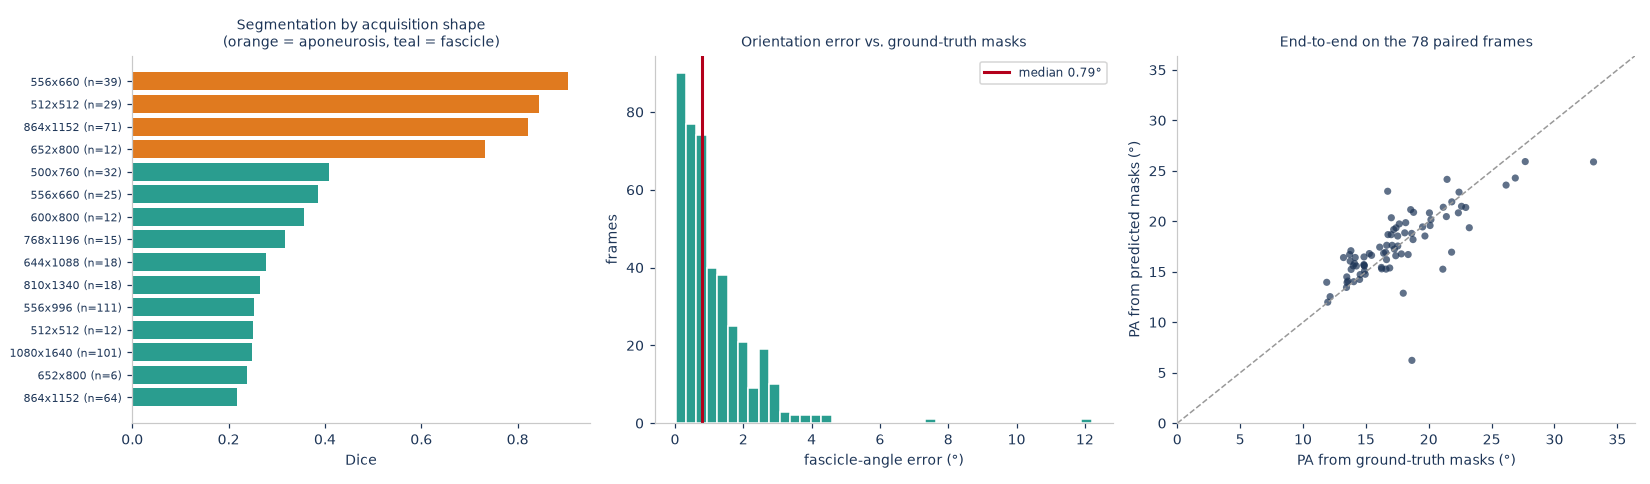
\includegraphics[width=\textwidth]{evaluation.png}
\caption{Held-out evaluation. Left: segmentation by acquisition shape.
Middle: fascicle-angle error against ground-truth masks. Right: pennation angle
from predicted versus annotator masks on the 78 paired frames.}
\label{fig:evaluation}
\end{figure}

\subsection{Generalisation across scanner families}
\label{sec:generalisation}

Aponeurosis Dice ranges from 0.732 to 0.905 across acquisition shapes, and
fascicle Dice from 0.218 to 0.408 --- close to a factor of two. The weakest
families are not the rarest, so this is not simply a data-quantity effect.
Predicted thickness also differs substantially by family, spanning
\SIrange{16.9}{29.1}{\milli\metre}. Some of that is genuine anatomy, since
different scanners were used for different muscles, but it cannot all be, and
with no per-family ground truth the two cannot be separated from inside this
competition. \textbf{This is the weakest link in the generalisation story} and
the most plausible home for the residual leaderboard gap.

\begin{figure}[htbp]
\centering
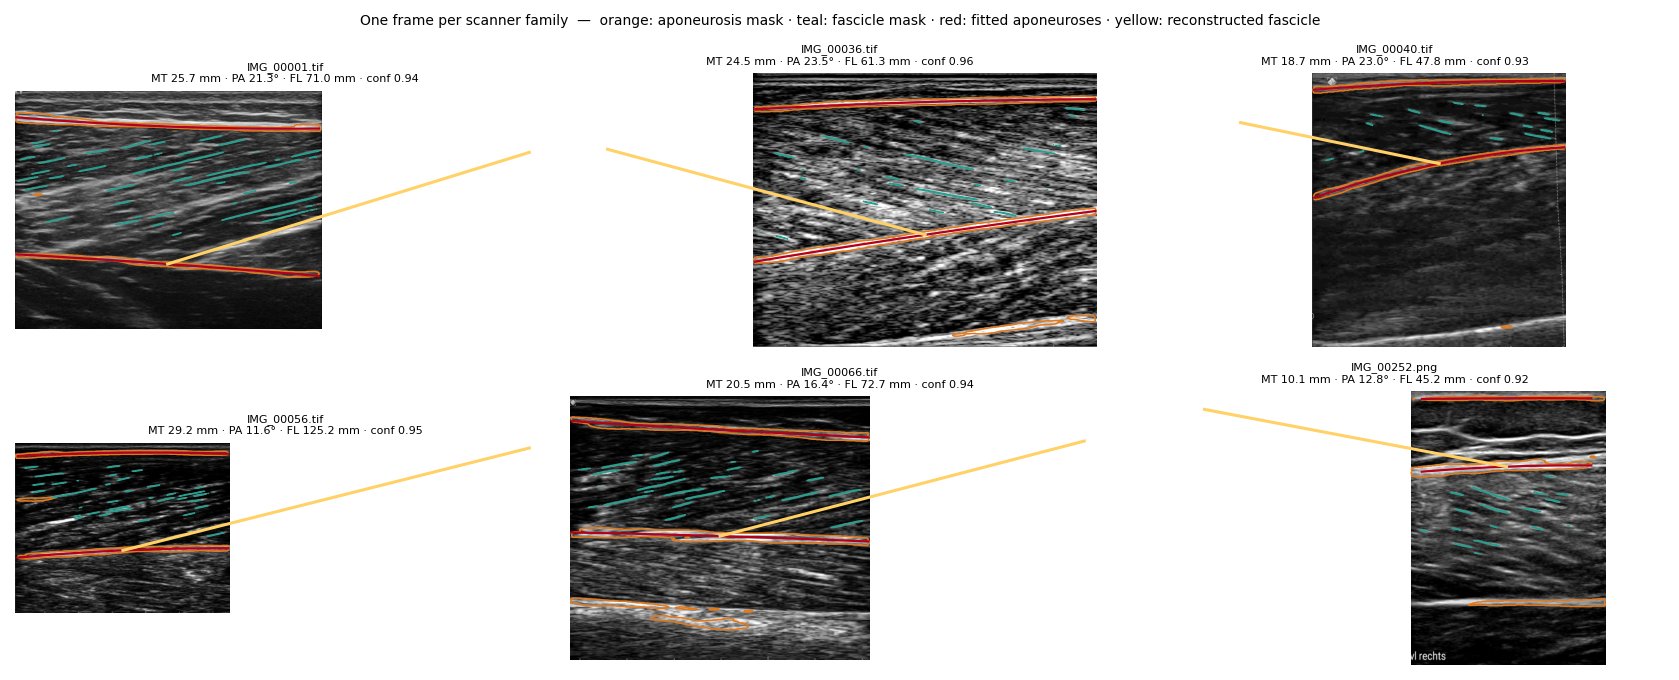
\includegraphics[width=\textwidth]{qualitative_by_device.png}
\caption{One test frame per scanner family. Orange: predicted aponeurosis mask.
Teal: predicted fascicle mask. Red: fitted aponeurosis curves. Yellow: the
reconstructed fascicle.}
\label{fig:qualitative}
\end{figure}

\subsection{Leaderboard}

\begin{table}[htbp]
\centering
\caption{Public leaderboard context (\texttt{UMUD\_score}, lower is better).}
\label{tab:lb}
\begin{tabular}{lr}
\toprule
\textbf{Entry} & \textbf{Public LB} \\
\midrule
Best public entry & 0.283 \\
Approximate median public entry & $\sim$0.40 \\
A published segmentation entry~\citep{dread2026vera} & 0.451 \\
\textbf{This pipeline} & \textbf{0.753} \\
DL\_Track\_US v0.3.1, the field's reference tool~\citep{ritsche2024dltrack} & 0.779 \\
A purely geometric, no-learning baseline~\citep{ambrosm2026quickdirty} & 1.339 \\
\bottomrule
\end{tabular}
\end{table}

The pipeline lands just ahead of the tool this field currently uses, and well
behind the strongest public entries. For a system built from scratch within the
project budget that is a reasonable position, and it is not a competitive result.

\subsection{Ablations}
\label{sec:disc}

Four mechanisms were proposed. Each was measured against the thing it replaced.
\textbf{Three did not earn their place, and the fourth works for a different
reason than proposed.} The measurements are reported as they came out.

\subsubsection{Fascicle length: the faithful model is the worse estimator}
\label{sec:abl-fl}

\begin{table}[htbp]
\centering
\caption{Fascicle-length construction, paired set ($n=78$) and leaderboard.}
\label{tab:abl-fl}
\begin{tabular}{lrr}
\toprule
\textbf{Construction} & \textbf{Median rel.\ error} & \textbf{Public LB} \\
\midrule
Intersection \eqref{eq:intersect} & 0.077 & 0.79372 \\
Textbook $\MT/\sin\PA$ \eqref{eq:textbook} & \textbf{0.060} & 0.81269 \\
\textbf{\texttt{auto} (selects between them)} & --- & \textbf{0.75306} \\
\bottomrule
\end{tabular}
\end{table}

On the paired set the textbook formula wins decisively: better on 68\,\% of
frames, Wilcoxon signed-rank $p=0.0003$. This contradicts the proposal's premise.

Crucially, the intersection does \emph{not} lose because divergence is estimated
badly --- it is recovered to \ang{0.15}. It loses because of what each formula
\emph{depends on}. The textbook formula leans on muscle thickness, recovered to
0.3\,\%; the intersection leans on the \emph{difference} of two fitted
aponeurosis angles and on the fascicle angle, inheriting angular noise twice
over. \textbf{A model that is more faithful in principle bought a worse answer in
practice by depending on noisier inputs.}

\paragraph{But the leaderboard disagreed --- and both were right.} Before
consulting it we recorded that a worse score would be read as ``the paired set
did not generalise'' rather than as licence to re-pick the winner. The
leaderboard then reversed the ordering. The explanation is a population mismatch:

\begin{table}[htbp]
\centering
\caption{Pennation-angle distributions. $\MT/\sin\PA$ diverges as $1/\sin$.}
\label{tab:pa-dist}
\begin{tabular}{lrr}
\toprule
& \textbf{Frames below \ang{12}} & \textbf{Minimum \PA} \\
\midrule
Paired evaluation set ($n=78$) & 3\,\% & \ang{11.9} \\
Test set ($n=309$) & \textbf{15\,\%} & \textbf{\ang{3.0}} \\
\bottomrule
\end{tabular}
\end{table}

At \ang{8}, \eqref{eq:textbook} predicts a \SI{167}{\milli\metre} fascicle. The
paired set contains almost none of that regime, so the divergence never bit
there. The intersection \emph{cannot} diverge --- the ray meets the superficial
aponeurosis at a finite distance --- so it degrades gracefully exactly where the
other fails.

The shipped default, \texttt{fl\_method="auto"}, therefore takes the textbook
value while it lands inside the physiological range and the intersection when it
does not. \textbf{This introduces no tuned parameter}: the bound it tests against
is the clamp the estimate would have hit anyway, and it is a no-op when the
aponeuroses are parallel, because the two constructions then coincide exactly. It
fired on \textbf{41 of 309} test frames --- exactly the set identified in advance
--- and improves the leaderboard by 5\,\% relative over the better pure
construction.

\textbf{Note what this does not vindicate.} The proposal argued for the
intersection from aponeurosis non-parallelism, and on that account it still loses
outright. It earns its place through \emph{boundedness} against $1/\sin$
ill-conditioning --- a different property the original reasoning never
identified. Right mechanism, wrong reason.

\subsubsection{Orientation head versus the post-processing it replaced}
\label{sec:abl-orientation}

\begin{table}[htbp]
\centering
\caption{Fascicle-angle error against annotator masks, held-out.}
\label{tab:abl-ori}
\begin{tabular}{lr}
\toprule
\textbf{Route} & \textbf{Median angular error} \\
\midrule
Dense orientation head (this project's contribution) & \ang{0.79} \\
Structure tensor on the predicted mask (classical) & \textbf{\ang{0.72}} \\
\bottomrule
\end{tabular}
\end{table}

The head does \emph{not} beat the post-processing it was designed to replace.
Both are accurate in absolute terms --- under a degree, against a \ang{45} chance
level --- but the proposal's argument was that predicting orientation
\emph{directly} is better than recovering it afterwards, and on this evidence it
is not. On this dataset the extra head is unjustified complexity.

\subsubsection{Sequence smoothing is nearly inert}

Within-run spread \emph{before} smoothing, across the 27 recovered runs:
\ang{0.14} in pennation angle, \SI{0.73}{\milli\metre} in fascicle length, and
\SI{0.02}{\milli\metre} in thickness. There is almost nothing to average away.
Recovering the run structure was a genuine finding about the data; exploiting it
was not worth much.

\subsubsection{Per-frame confidence does not predict error}

Spearman correlations between confidence and error are $-0.08$ (\PA), $-0.17$
(\FL) and $-0.19$ (\MT): correctly signed, but weak and not significant at
$n=78$. \textbf{The confidence is not a usable uncertainty estimate.}

This carried a methodological trap worth recording. An earlier version multiplied
the confidence by 0.6 whenever an estimate hit a physiological clamp, which made
it \emph{appear} to detect failures: clamped frames showed median confidence
0.564 against $0.6\times0.934=0.560$ for the rest --- the entire gap was the
penalty, and the independent components did not discriminate at all. The
confidence was not predicting the failure; it was being told about it. The term
was removed and a regression test now pins the invariant that confidence may use
only evidence available \emph{before} the estimate exists.

\subsection{Limitations}

\begin{enumerate}
  \item \textbf{No expert-measurement validation.} Every offline number compares
        the pipeline against annotator \emph{masks} through the same geometry
        module. Systematic error in the geometry module itself is invisible to
        this protocol.
  \item \textbf{The scale is trusted, not verified.} Calibration covers 100\,\%
        of test frames and the implied fields of view are plausible, but nothing
        independently confirms any individual frame was read correctly.
  \item \textbf{The paired set is small and homogeneous.} All 78 frames come from
        one scanner family --- a limitation that Section~\ref{sec:abl-fl} shows
        materially changed a conclusion.
  \item \textbf{Fascicle length is extrapolated, not observed.} Annotations cover
        10--20\,\% of a fascicle. Every \FL{} value assumes local straightness;
        curved fascicles will be mis-measured and this protocol cannot detect it.
  \item \textbf{Physiological clamping hides failures} by converting a detectable
        failure into a plausible-looking wrong answer.
  \item \textbf{Single split, single seed.} The compute budget allowed one
        training run per task, so small differences between ablation arms should
        not be over-read.
\end{enumerate}

\subsection{Future work}

Calibrating uncertainty against the UMUD multi-expert set (35 frames, six
raters); a genuine temporal module on UMUD video data using
RAFT~\citep{teed2020raft}; fine-tuning SAM~\citep{kirillov2023sam} as a
segmentation backbone; and closing the per-family gap identified in
Section~\ref{sec:generalisation}, which is where the remaining leaderboard
distance most plausibly lies.

\section{Conclusion}

We built an automatic muscle-architecture estimator that scores 0.753 on the UMUD
public leaderboard, ahead of the field's reference tool, recovering muscle
thickness to 0.3\,\% and pennation angle to \ang{1.16} against annotator masks.
The engineering that mattered most was not the deep learning but the recovery of
physical scale from the scanner's own ruler --- a component the original proposal
never contemplated, because it assumed the measurements were learnable targets.

Of the four mechanisms actually proposed, one was refuted outright, one turned
out to help for a reason the proposal did not identify, one proved nearly inert,
and one could not be attempted with the available data. We consider this the
most useful outcome of the project: in particular, the finding that a more
faithful geometric model can be a worse estimator when it depends on noisier
inputs is a lesson that transfers well beyond muscle ultrasound.

%-------------------------------------------------------------- REFERENCES ---
\bibliographystyle{plainnat}
\bibliography{references}

\appendix
\section{Reproducibility}

All training and inference ran on Kaggle GPU kernels; nothing heavy runs locally.
The repository at \url{https://github.com/silvererudite/umud-muscle-architecture}
contains the full pipeline, 27 unit tests, an executed exploratory notebook, and
both Kaggle kernels. A complete run is:

\begin{verbatim}
export KAGGLE_API_TOKEN=...
./scripts/run_pipeline.sh "run description"
\end{verbatim}

which ships the source package as a Kaggle dataset, trains both networks, runs
inference, evaluation and ablations, rebuilds every results figure, validates the
submission, and submits it.

\end{document}
